% !TeX document-id = {acd94374-0a5a-4c39-a15c-8f2e56f0151a}
\documentclass[12pt,a4paper, listof=entryprefix, bibliography=totocnumbered,toc=listofnumbered,lof=listofnumbered]{scrartcl}

% WICHTIG!!!
% Pseudokommentar um pdflatex zu erlauben andere Programme zu nutzen z.B. gnuplot
% !TeX TXS-program:compile = txs:///pdflatex/[--shell-escape] 

\usepackage[ngerman]{babel}
\usepackage[utf8]{inputenc}
\usepackage{amsmath}
\usepackage{nccmath}
\usepackage{amsfonts}
\usepackage{amssymb}
\usepackage{graphicx}
\usepackage{fancyhdr}
\usepackage{tabularx}
\usepackage{geometry}
\usepackage{setspace}
\usepackage[right]{eurosym}
\usepackage[printonlyused]{acronym}
\usepackage{subfig}
\usepackage{floatflt}
\usepackage[usenames,dvipsnames]{color}
\usepackage{colortbl}
\usepackage{xcolor}
\usepackage{paralist}
\usepackage{array}
\usepackage{titlesec}
\usepackage{parskip}
\usepackage{picinpar}
\usepackage[pdfpagelabels=true]{hyperref}
\usepackage{listings}
\usepackage{csquotes}
\usepackage{url}
\usepackage{float}
\usepackage{pgfplots}
\usepackage{paralist}
\usepackage[nonumberlist, nogroupskip]{glossaries}

%-----------------------------------------------------------------------------------
% Bibilothek
%-----------------------------------------------------------------------------------
% Einbinden des BibLateX paketes mit Ausgabeeinstellungen
\usepackage[
style=alphabetic,          % Zitierstil
maxbibnames=50,            % alle Autorennamen anzeigen
maxcitenames=4,            % maximale Namen, die im Kürzel angezeigt werden
autocite=inline,           % regelt Aussehen für \autocite (inline=\parancite)
block=space,               % kleiner horizontaler Platz zwischen den Feldern
backref=true,              % Seiten anzeigen, auf denen die Referenz vorkommt
backrefstyle=three+,       % fasst Seiten zusammen, z.B. S. 2f, 6ff, 7-10
date=short,                % Datumsformat
backend = biber,           % Backnend für Aufbereitung
]{biblatex}

%Zusätzliche für Umbrüche für Kleinbuchstaben z.B. in URLs
\appto\UrlBreaks{\do\a\do\b\do\c\do\d\do\e\do\f\do\g\do\h\do\i\do\j
	\do\k\do\l\do\m\do\n\do\o\do\p\do\q\do\r\do\s\do\t\do\u\do\v\do\w
	\do\x\do\y\do\z}


\newcounter{verzeichnis}
\setcounter{verzeichnis}{1}

%Abstände der Einträge
\setlength{\bibitemsep}{1em}     % Abstand zwischen den Literaturangaben
\setlength{\bibhang}{2em}        % Einzug nach jeweils erster Zeile

% Kürzel soll vier Buchstaben der Autoren enthalten statt drei
\DeclareLabelalphaTemplate{
	\labelelement{
		\field[final]{shorthand}
		\field{label}
		\field[strwidth=4,strside=left,ifnames=1]{labelname}
		\field[strwidth=2,strside=left,ifnames=2]{labelname}
		\field[strwidth=1,strside=left]{labelname}
	}
	\labelelement{
		\field[strwidth=2,strside=right]{year}
	}
}

% Bibliothek der Quellen
\bibliography{bib}
\label{bib}

% --------------------------------------------------------------------------------
% Einstellung für Listings
% --------------------------------------------------------------------------------
\lstset{basicstyle=\footnotesize, captionpos=b, breaklines=true, showstringspaces=false, tabsize=2, frame=lines, numbers=left, numberstyle=\tiny, xleftmargin=2em, framexleftmargin=2em}
\makeatletter
\def\l@lstlisting#1#2{\@dottedtocline{1}{0em}{1em}{\hspace{1,5em} Lst. #1}{#2}}
\makeatother

% --------------------------------------------------------------------------------
% Seitenformate
% --------------------------------------------------------------------------------
%Seitenformat
\geometry{a4paper, top=27mm, left=30mm, right=20mm, bottom=32mm, headsep=12mm, footskip=12mm}

% --------------------------------------------------------------------------------
% Metainformationen
% --------------------------------------------------------------------------------
\hypersetup{unicode=false, pdftoolbar=true, pdfmenubar=true, pdffitwindow=false, pdfstartview={FitH},
	pdftitle={Vorlage},
	pdfauthor={Stefan Jung},
	pdfsubject={Abschlussarbeit},
	pdfcreator={\LaTeX\ with package \flqq hyperref\frqq},
	pdfproducer={pdfTeX \the\pdftexversion.\pdftexrevision},
	pdfkeywords={Vorlage},
	pdfnewwindow=true,
	colorlinks=true,linkcolor=black,citecolor=black,filecolor=magenta,urlcolor=black}
\pdfinfo{/CreationDate (D:20141024101000)}
\pgfplotsset{compat=1.11}

%-----------------------------------------------------------------------------------
% Abkürzungen AKRONYME HIER ERGÄNZEN
%-----------------------------------------------------------------------------------
\glssetwidest{SMPLSP}% Längste Abkürzung für eine korrekte Einrückung

\makenoidxglossaries %Leeres Verzeichnis erstellen

%Abkürzungen hinzufügen
\newacronym{LIP}{LIP}{Labor für Informationstechnik und Produktionslogistik}
\newacronym{JRE}{JRE}{Java Runtime Environment}
\newacronym{SMPLSP}{SMPLSP}{Static Multi-Product Proportional Lotsizing and Scheduling Problem}
\newacronym{OTH}{OTHR}{Ostbayerische Technische Hochschule Regensburg}

\begin{document}
% --------------------------------------------------------------------------------
% Globale Formateinstellungen
% --------------------------------------------------------------------------------
\onehalfspacing
% Abstände Überschrift
\titlespacing{\section}{0pt}{42pt}{6pt}
\titlespacing{\subsection}{0pt}{12pt}{6pt}
\titlespacing{\subsubsection}{0pt}{12pt}{6pt}

% Kopf- und Fusszeile
\pagestyle{fancy}
\lhead{}\chead{}
\rhead{\thesection\space\contentsname}
\lhead{}\cfoot{}
\rfoot{\ \linebreak \thepage}
\renewcommand{\headrulewidth}{0.4pt}
\renewcommand{\footrulewidth}{0.4pt}

% Nummereriung
\renewcommand{\thesection}{\Roman{section}}
\renewcommand{\theHsection}{\Roman{section}}
\pagenumbering{Roman}

% eigene Farbdefinitionen
\definecolor{lip}{HTML}{3366FF}
\definecolor{grey}{HTML}{ABABAB}

% ---------------------------------------------------------------------------
% Titelseite
% ---------------------------------------------------------------------------
\thispagestyle{empty}

%LIP Schriftzug in eigener Farbe 
\textsf{\begin{minipage}{.69\textwidth}
	\large
	\textcolor{lip}{\textbf{Labor für Informationstechnik und\\Produktionslogistik (LIP)}} %Farbe setzten
	\small 
	\textbf{\\Verfahren, Strategien, Prozesse und IT-Systeme}
	\\Professor Dr.-Ing. Frank Herrmann
\end{minipage}
%Einbinden des OTH Logos mir rechtsbündiger Ausrichtung
\begin{minipage}{.29\textwidth}
	\begin{flushright}
		
\includegraphics[scale=.15]{Bilder/othlogo}\\
	\end{flushright}
\end{minipage}}
 
% Zeilenabstand
\onehalfspacing	

%Beschriftung der Titelseite
\begin{center}

	\vspace*{4cm} %4 cm Vorspann
	\Large
	\textbf{Benutzerhandbuch zur Losgrößen- und Ressourceneinsatzplanung bei Fließproduktion}\\ %Titel der Arbeit
	\large
	\textbf{Klassisches Losgrößenmodell, Mehrproduktproduktion}\\ %Untertitel der Arbeit
		
	\vspace*{8cm} %8 cm Vorspann
	\normalsize
	\begin{center}
	Aktueller Stand: \today 
	
	\textbf{Christiane Arnold\\Timo Denzin\\Tobias Eichinger\\Daniel Sonnleitner\\Pilar Wagner} %Name des Autors
	
	\end{center}
\end{center}
\pagebreak

% ------------------------------------------------------------------------------
% Inhaltsverzeichnis
% ------------------------------------------------------------------------------
% Inhaltsverzeichnis
\singlespacing %Zeilenabsatnd reduzieren
\setcounter{section}{0}
\setcounter{page}{1}
\addcontentsline{toc}{section}{Inhaltsverzeichnis}%hinzufügen des Inhaltsverzeichnises selbst

\tableofcontents %Ausgabe des Inhaltsverzeichnisses
\pagebreak

% ------------------------------------------------------------------------------
% Setzen der Nummerierungen für Normaltext
% ------------------------------------------------------------------------------
\onehalfspacing %Zeilenabstand auf 1.5
\renewcommand{\thesection}{\arabic{section}} %Arabische Beschriftung für Absatznummern
\pagenumbering{arabic}  %Seitennummerrierung auf arabisch setzten
\setcounter{page}{1}	%Seitenzahl für Inhalt auf 1 setzten
\setcounter{section}{0}
% Kopfzeile mit aktuellem Hauptkapitel darstellen
\renewcommand{\sectionmark}[1]{\markright{#1}} %Section ausgeben
\renewcommand{\subsectionmark}[1]{}            %Subsection nicht ausgeben
\renewcommand{\subsubsectionmark}[1]{}         %Subsubsection nicht ausgeben
\rhead{\rightmark}                             %Ausgabe Rechtsbündig

%------------------------------------------------------------------------------
%	Einfuehrung
%------------------------------------------------------------------------------
\section{Einführung}
\label{ch:einfuehrung}
Das vorliegende Dokument beschreibt die Handhabung und Funktionsweise der Software \gls{SMPLSP} zur Losgrößen- und Ressourceneinsatzplanung bei Fließproduktion. \\
Das Tool wurde im Rahmen des Projektstudium 1 (Hauptseminar 1) im Masterstudiengang Informatik bei Herrn Professor Dr.-Ing. Frank Herrmann entwickelt und soll den Studenten
eine Möglichkeit bieten, das im Buch „Produktion und Logistik“ von Günther und Tempelmeier \cite{Templ09} gezeigte Verfahren zur Losgrößen- und Ressourceneinsatzplanung bei Fließproduktion nachzuvollziehen.
Umgesetzt wurden sowohl das klassische Losgrößenverfahren, als auch die Losgrößenberechnung bei Mehrproduktproduktion.

\subsection{Klassisches Losgrößenverfahren}
Das klassische Losgrößenverfahren betrachtet die Herstellung mehrerer Produkte auf einer
einzelnen Produktionsanlage. Da die Berechnung der optimalen Losgröße und des optimalen
Produktionszyklus für jedes Produkt isoliert durchgeführt werden kann es zu einer zeitlichen Überschneidung der Produktionsaufträge kommen. Daher ist die Produktion mehrerer Produkte unter Einhaltung des berechneten Produktionsplans aus dem klassischen Losgrößenverfahren häufig nicht möglich. Eine Fallstudie zu diesem Verfahren ist in \cite{Templ09} verfügbar.

\subsection{Mehrproduktproduktion}
Das Problem der Überschneidung von Produktionsaufträgen bei der Mehrproduktproduktion auf einer Anlage lässt sich durch die Bestimmung eines für alle Produkte einheitlichen gemeinsamen Produktionszyklus vermeiden. Die Aufgabe dieses Verfahrens ist die Bestimmung eines solchen gemeinsamen Produktionszyklus, sowie die Berechnung der optimalen Losgröße je Produkt. Eine Fallstudie zu diesem Verfahren ist in \cite{Templ09} verfügbar.
\pagebreak

%------------------------------------------------------------------------------
%	Installation
%------------------------------------------------------------------------------
\section{Installation}
\label{ch:installation}
%Das Tool benötigt das \gls{JRE}. Hierfür ist eine funktionierende \gls{JRE} Installation (Java 8) notwendig. Um das Programm auch ohne eine \gls{JRE} Installation ausführen zu können, werden verschiedene Dateien ausgeliefert:
Um das Programm auf verschiedenen Systemen ausführen zu können, werden mehrere Varianten
ausgeliefert:
\begin{compactitem}
	\item SMPLSP.jar \\
	Die .jar Datei kann durch Doppelklick verwendet werden, sofern auf dem Computer Java 8 installiert ist.
	\item SMPLSP-Installer.exe \\
	Für den Fall, dass kein Java 8 auf dem Computer installiert sein sollte, wird die .exe Datei ausgeliefert, welche das Programm nach Ausführung durch Doppelklick installiert und öffnet. Der Installationspfad "'C:\textbackslash Users\textbackslash Username\textbackslash AppData\textbackslash Local\textbackslash SMPLSP"' kann nicht verändert werden. Das Programm kann anschließend im Windows-Explorer oder über das Start-Menü aufgerufen werden.
\item SMPLSP.exe \\
Sollte kein Java 8 installiert und keine Installation des Programms auf dem Rechner gewünscht sein, kann das Programm durch Doppelklick auf die SMPLSP.exe ausgeführt werden.
	\item SMPLSP.dmg \\
	Diese Datei ermöglicht die Ausführung des Programms unter MAC OS.
\end{compactitem}

\pagebreak

%------------------------------------------------------------------------------
%	Programmablauf
%------------------------------------------------------------------------------
\section{Programmablauf}
\label{ch:programmablauf}
Im Folgenden wird der komplette Programmablauf mit allen möglichen Funktionen erläutert.

\subsection{Allgemein}
Das Tool enthält einige Komponenten/Abläufe, welche im Programm an mehreren Stellen in gleicher Weise auftreten.

\subsubsection{Programmeingaben}
\label{ch:programmeingaben}
Die Eingabe der Programmparameter erfolgt in Tabellenform (siehe Abbildung \ref{fig:benutzereingabe} a). Hierbei entspricht jede Zeile einem Produkt mit den zugehörigen Parametern (Spalten). Die Produkte werden zur Identifizierung automatisch mit einem fortlaufendem Index k (erste Spalte) belegt. Zur Durchführung der beiden Verfahren werden dabei pro Produkt folgende Parameter benötigt:
\begin{compactitem}
	\item Nachfragerate D
	\item Produktionsrate p
	\item Rüstzeit $\tau$
	\item Rüstkostensatz s
	\item Lagerkostensatz h
\end{compactitem}
Hinweise zu den einzelnen Eingabeparametern können der Erklärkomponente im unteren Teil der Benutzeroberfläche (siehe Abbildung \ref{fig:benutzereingabe} h), sowie dem Tooltip entnommen werden.

Zur Eingabe von Werten für die benötigten Programmparameter sind folgende Optionen vorgesehen:
\begin{compactitem}
	\item Händische Eingabe der Programmparameter
	\item Import der Programmparameter
	\item Laden von Testdaten
\end{compactitem}
\begin{figure}[H]
	\centering
	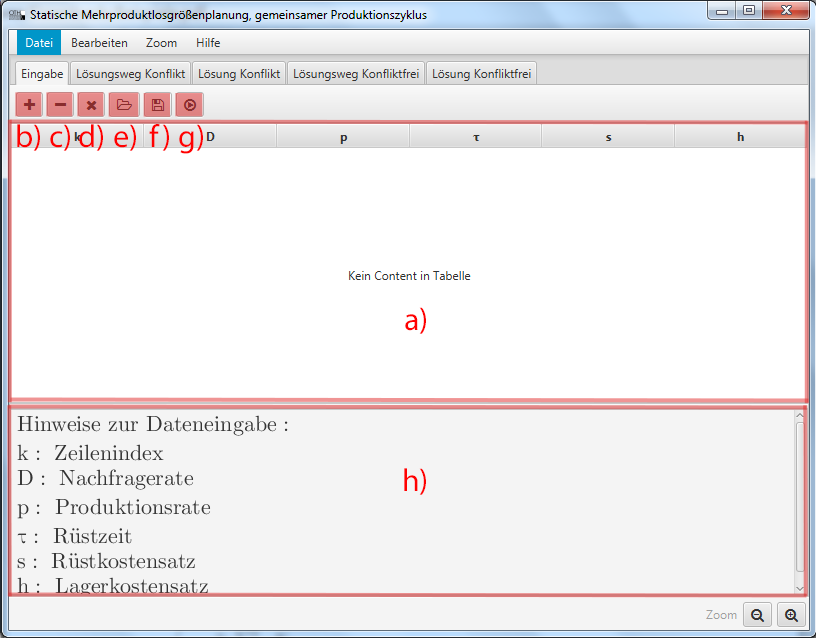
\includegraphics[width=0.8\linewidth]{Bilder/Benutzereingabe1.png} 
	\captionof{figure}[Benutzereingabe]{Startseite des Programms/Benutzereingabe}
	\label{fig:benutzereingabe}
\end{figure}

\paragraph{Händische Eingabe der Programmparameter:}~\\
Für das \textbf{Hinzufügen von Produkten} muss zuerst durch einen einfachen Klick auf das "'+"'-Symbol (siehe Abbildung \ref{fig:benutzereingabe} b) in der Toolleiste oberhalb der Tabelle (siehe Abbildung \ref{fig:benutzereingabe}) eine neue Zeile hinzugefügt werden. Jede neu eingefügte Zeile wird automatisch mit einem nicht veränderbaren Zeilenindex k belegt. Durch Doppelklick auf die einzelnen Spalten können Werte hinzugefügt werden. Eine Alternative zum Hinzufügen einer neuen Zeile über das "'+"'-Symbol stellt der Eintrag "'Hinzufügen"' im Menüreiter "'Bearbeiten"' bereit.

Zum \textbf{Löschen von Produkten} wird die entsprechende Tabellenzeile markiert und anschließend durch einen Klick auf das „-“ - Symbol (siehe Abbildung \ref{fig:benutzereingabe} c) aus der Tabelle entfernt. Sollte zum Zeitpunkt des Klicks keine Zeile markiert sein wird dies dem Benutzer durch einen Warndialog, dargestellt in Abbildung \ref{fig:keineauswahl}, mitgeteilt. Eine Alternative zum Löschen einer Zeile über das "'-"'-Symbol stellt der Eintrag "'Löschen"' im Menüreiter "'Bearbeiten"' bereit.
\begin{figure}[H]
	\centering
	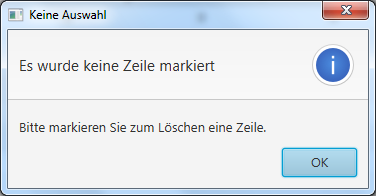
\includegraphics[width=0.5\linewidth]{Bilder/KeineZeilenAuswahl.png} 
	\captionof{figure}[Keine Zeilenauswahl]{Warnhinweis: Keine Zeilenauswahl}
	\label{fig:keineauswahl}
\end{figure}
Das \textbf{Löschen der gesamten Tabelleninhalte} ist durch Klick auf das "'X"'-Symbol (siehe Abbildung \ref{fig:benutzereingabe} d) möglich. Bevor die gesamten Tabelleninhalte gelöscht werden, wird der Benutzer zu einer Bestätigung der gewünschten Aktion durch einen entsprechenden Dialog (siehe Abbildung \ref{fig:datenloeschen}) angehalten. Mit Klick auf den "'Abbrechen"'-Button wird die Aktion abgebrochen und die Daten nicht gelöscht. Eine Alternative zum Löschen sämtlicher Tabelleninhalte über das "'X"'-Symbol stellt der Eintrag "'Alles Löschen"' im Menüreiter "'Bearbeiten"' bereit.
\begin{figure}[H]
	\centering
	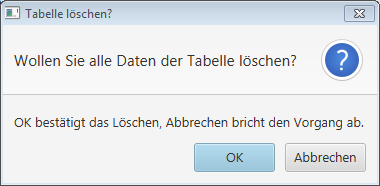
\includegraphics[width=0.5\linewidth]{Bilder/DatenLoeschen.png} 
	\captionof{figure}[Alle Daten löschen]{Warnhinweis: Alle Daten löschen}
	\label{fig:datenloeschen}
\end{figure}

\paragraph{Import der Programmparameter:}~\\
CSV-Dateien können durch Klick auf das Ordnersymbol (…) ausgewählt und importiert werden (siehe Abbildung \ref{fig:benutzereingabe} e). Alternativ kann der Öffnen-Dialog über den Shortcut "'Strg o"' erreicht werden. Sollten bereits Daten in der Tabelle eingetragen sein, so wird der Benutzer gefragt ob die Daten überschrieben werden sollen. Eine Alternative Aufrufmöglichkeit besteht in der Menüleiste unter "Datei".

Das \textbf{Exportieren von Eingabeparametern} wird durch Klick auf das "'Speichern"'-Symbol (siehe Abbildung \ref{fig:benutzereingabe} f) oder den Shortcut "'Strg s"' ausgelöst. Nach Auswahl eines geeigneten Speicherorts wird die Tabelle im CSV-Format abgespeichert. Eine Alternative Aufrufmöglichkeit besteht in der Menüleiste unter "Datei".

\paragraph{Laden von Testdaten:}~\\
Für einen schnellen Einstieg in die Nutzung des Programms, ist es möglich Testdaten zu laden. Hierfür muss im Menüeintrag "'Datei"' auf "'Testdaten laden"' geklickt oder die Tastenkombination "'Strg t"' gedrückt werden. Die Testdaten entsprechen den Daten aus der in \cite{Templ09} vorgestellten Fallstudie.

\paragraph{Starten der Berechnung:}~\\
Die Berechnung wird durch einen Klick auf das "'Berechnen"'-Symbol (siehe Abbildung \ref{fig:benutzereingabe} g) oder mit der Tastenkombination "'Strg b"' gestartet. Um die Berechnung erfolgreich durchführen zu können ist es notwendig, dass alle Eingabeparameter mit einem Wert größer Null belegt sind. Ist dies nicht der Fall, wird der Benutzer durch einen Dialog aufgefordert die fehlenden Werte zu ergänzen (siehe Abbildung \ref{fig:ungueltigewerte}). 

\begin{figure}[H]
	\centering
	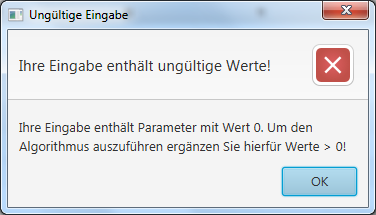
\includegraphics[width=0.5\linewidth]{Bilder/UngueltigeWerte.png} 
	\captionof{figure}[Ungültig Eingabewerte]{Warnhinweis: Ungültig Eingabewerte}
	\label{fig:ungueltigewerte}
\end{figure}

Schlägt die Berechnung aus einem anderen Grund fehl, wird dies dem Benutzter in einem
Fehlerdialog angezeigt.

\subsubsection{Allgemeine Funktionen}
Im Nachfolgenden werden die Funktionen, welche über den gesamten Programmablauf hin genutzt werden können, erläutert.

\paragraph{Einstellungen:}~\\
\label{par:einstellungen}
Die Einstellungen sind über den Menüreiter "'Datei"' erreichbar. Von hier aus kann das Programm bezüglich der darzustellenden Nachkommastellen und der Farbeinstellungen angepasst werden (siehe Abbildung \ref{fig:einstellungen}). Durch Bestätigen der Änderungen über den "'Speichern"'-Button oder mit der Enter-Taste werden die geänderten Werte übernommen.

Die \textbf{Eingabe der Nachkommastellen} bewirkt eine Anpassung der Nachkommastellen bei sämtlichen Zahlen innerhalb der Applikation. Während die Berechnung mit den Originalzahlen durchgeführt wird, wird die Darstellung durch Runden auf die gewünschte Anzahl Nachkommastellen verändert. 

Die \textbf{Anpassung der Farbeinstellung} kann durch Setzen, bzw. Entfernen des Häkchens "'Schwarz/Weiß"' vorgenommen werden. Der Schwarz/Weiß Modus bietet einen starken Kontrast und ist daher für den Einsatz am Beamer geeignet. Zu Lernzwecken ist der Farbmodus zu bevorzugen, da hier eine farbliche Zuordnung zwischen Eingabeparametern und Formeln erfolgt.

\begin{figure}[H]
	\centering
	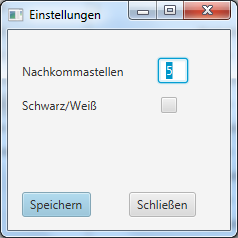
\includegraphics[width=0.3\linewidth]{Bilder/Einstellungen.png} 
	\captionof{figure}[Einstellungen]{Einstellungen}
	\label{fig:einstellungen}
\end{figure}

\paragraph{Zoomfunktionen:}~\\
Die Zoomfunktion wird durch die beiden Lupen-Buttons in der unteren rechten Ecke der Applikation aufgerufen werden (siehe Abbildung \ref{fig:zoom}). Dabei steht "'+"' für hinein- und "'-"' für herauszoomen. Hierbei werden alle Applikationselemente vollständig vergrößert bzw. verkleinert, wodurch die Applikation auch aus größerer Entfernung, wie z.B. bei Einsatz eines Beamers gut erkennbar ist. Die Zoom-Funktion kann ebenfalls über den Menüpunkt "'Zoom"' oder über die gängigen Shortcuts "'Strg +"' und "'Strg -"' angesteuert werden. Über den Eintrag "'Zoom zurücksetzen"' oder die Tastenkombination "'Strg 0"' kann der Zoom vollständig zurückgesetzt werden.
\begin{figure}[H]
	\centering
	
\includegraphics[width=0.3\linewidth]{Bilder/Zoom.png} 
	\captionof{figure}[Zoomfunktionen]{Zoomfunktionen}
	\label{fig:zoom}
\end{figure}

\paragraph{About:}~\\
Der About ("'Über"') Dialog kann über den Menüpunkt "'Hilfe"' erreicht werden und liefert Informationen über die Software, sowie ihre Entwickler.

\subsection{Klassische Losgrößenplanung}
\label{ch:klassischeberechnung}
Die Lösungswerte der klassischen Losgrößenberechnung werden mit Hilfe der Formeln aus \cite{Templ09} berechnet.

Die Darstellung der Lösungswerte erfolgt im Reiter "'Lösungsweg Konflikt"'. Die Benutzeroberfläche ist wie folgt gegliedert:

\begin{compactitem}
	\item Tabelle mit den Lösungswerten für die optimale Losgröße, der daraus resultierenden Produktionsdauer und der Reichweite der einzelnen Produkte(siehe Abbildung \ref{fig:klassich} a)
	\item Tabelle mit Produktionsablauf (siehe Abbildung \ref{fig:klassich} b)
	\item Darstellung der Berechnung der einzelnen Lösungswerte in der Erklärkomponente (siehe Abbildung \ref{fig:klassich} c)
\end{compactitem}

Hinweise zu den einzelnen Spalten werden in der jeweiligen Tabelle als Tooltip angezeigt.  Die Darstellung der Berechnung in der Erklärkomponente wird durch das einfache Klicken auf eine Zeile einer Tabelle ausgelöst. Innerhalb einer Tabelle kann mit den Pfeiltasten der Tastatur navigiert werden. In der Erklärkomponente wird die allgemeine Lösungsformel sowie die Formel mit eingesetzten Werten für das gewählte Produkt angezeigt. Hierbei lässt sich eine farbliche Zuordnung der konkreten, eingesetzten Werte zu den in der Formel verwendeten Variablen herstellen, sofern der Schwarz-Weiß-Modus nicht aktiviert ist (siehe Einstellungen, Kapitel \ref{par:einstellungen}). 

\begin{figure}[H]
	\centering
	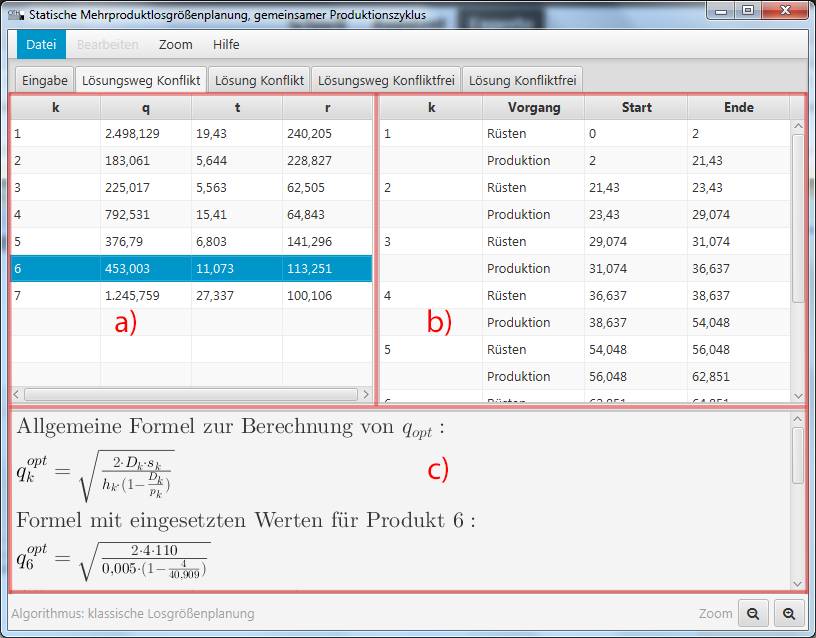
\includegraphics[width=0.8\linewidth]{Bilder/KlassischesVerfahren.png} 
	\captionof{figure}[Klassisches Losgrößenverfahren]{Klassisches Losgrößenverfahren - Darstellung der Lösungswerte}
	\label{fig:klassich}
\end{figure}

%Das in Reiter "'Lösung Konflikt"' dargestellte Gantt Chart (siehe Abbildung \ref{fig:ganttklassisch}) stellt eine graphische Aufarbeitung des Produktionsablauf aus Reiter "'Lösungsweg Konflikt"' dar, wobei auf der x-Achse die Zeit und auf der y-Achse die Produktindizes aufgetragen sind. Die Belegung der Anlage durch mehrere Produkte wird in der Zeile "'Überschneidung"' farblich markiert (rot) angezeigt.
Im Reiter „Lösung Konflikt“ wird der Produktionsablauf mittels eines Gantt Charst grafisch dargestellt. Auf der X-Achse ist die Zeit angetragen, auf der Y-Achse die Produktindizes. Folgendes Bild zeigt das Diagramm. Die rot gefärbten Balken zeigen die Konflikte zwischen den Produkten an.

Durch Klicken auf das Diagramm und ziehen der Maus nach rechts wird der ausgewählte Bereich vergrößert. Durch Klicken auf das Diagramm und ziehen der Maus nach links zeigt das Diagramm wieder den Originalbereich an. Alternativ genügt zum Anzeigen des Originalbereichs auch ein Klick in den Randbereich   des Charts.

\begin{figure}[H]
	\centering
	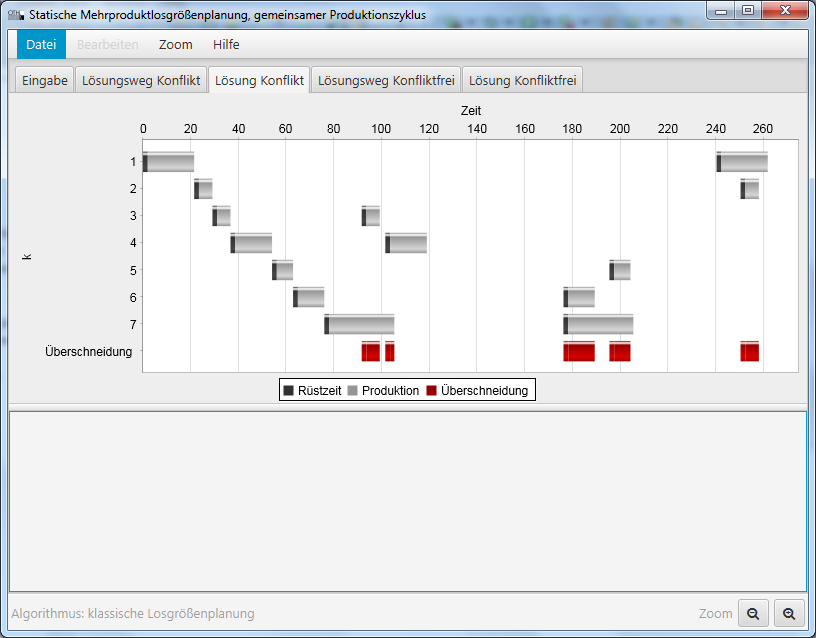
\includegraphics[width=0.8\linewidth]{Bilder/GanttKlassisch.png} 
	\captionof{figure}[Gantt Chart - klassische Losgrößenplanung]{Gantt Chart- Graphische Darstellung der Lösungswerte der klassischen Losgrößenplanung}
	\label{fig:ganttklassisch}
\end{figure}

\subsection{Mehrprodukt-Losgrößenplanung}
Ebenso wie die Lösungswerte der klassischen Losgrößenberechnung werden die Lösungswerte der Mehrprodukt-Losgrößenplanung mit Hilfe der Formeln aus \cite{Templ09} berechnet. Als Eingangsparameter für dieses Verfahren werden die Eingabeparameter im Reiter "'Eingabe"' verwendet. Es sind keinerlei Anpassungen zu machen. 

Es ist bei diesem Verfahren zu beachten, dass der berechnete optimale gemeinsame Produktionszyklus größer oder gleich dem berechneten minimalen Produktionszyklus sein muss. Ist dies nicht der Fall, wird der Benutzer nach Start der Berechnung darauf hingewiesen und dazu aufgefordert die Benutzereingabe dementsprechend anzupassen. Es erfolgt in diesem Fall keine Anzeige der Lösungswerte.

Nach erfolgreicher Berechnung erfolgt die Darstellung der Lösungswerte im Reiter "'Lösungsweg Konfliktfrei"', da dieses Verfahren zu einem überschneidungsfreien und somit ausführbaren Produktionsablaufplan führt. Die Benutzeroberfläche ist wie folgt gegliedert:

\begin{compactitem}
\item Allgemeine Lösungsformeln zur Berechnung des optimalen, gemeinsamen sowie des minimalen Produktionszyklus (siehe Abbildung \ref{fig:mehrprodukt} a)
	\item Tabelle mit den Lösungswerten für die optimale Losgröße, der daraus resultierenden Produktionsdauer und der Reichweite der einzelnen Produkte (siehe Abbildung \ref{fig:mehrprodukt} b)
	\item Tabelle mit Produktionsablauf (siehe Abbildung \ref{fig:mehrprodukt} c)
	\item Darstellung der Berechnung der einzelnen Lösungswerte in der Erklärkomponente (siehe Abbildung \ref{fig:mehrprodukt} d)
\end{compactitem}

Hinweise zu den einzelnen Spalten werden in der jeweiligen Tabelle als Tooltip angezeigt.  Die Darstellung der Berechnung in der Erklärkomponente und die Navigation innerhalb der Tabellen erfolgt wie beim klassischen Losgrößenverfahren in Abschnitt \ref{ch:klassischeberechnung}.
\begin{figure}[H]
	\centering
	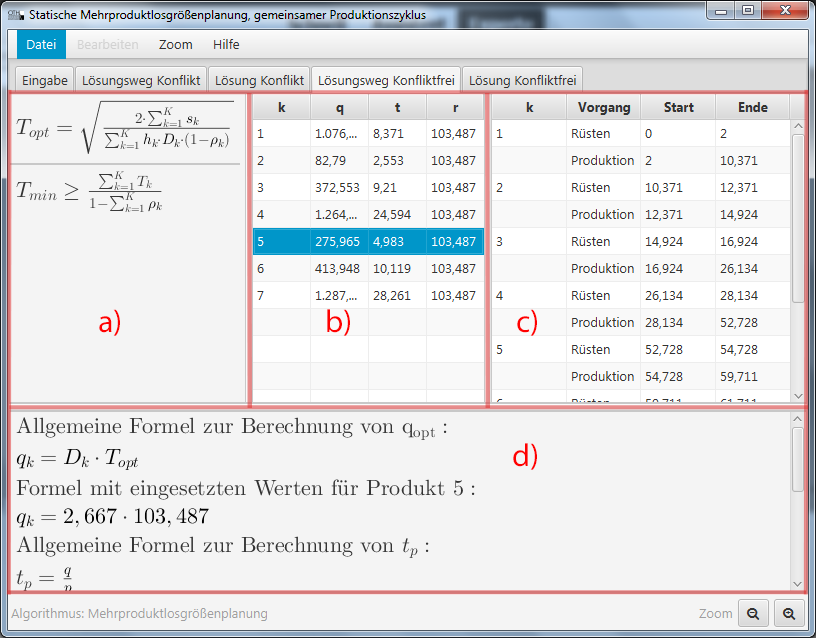
\includegraphics[width=0.8\linewidth]{Bilder/Mehrprodukt.png} 
	\captionof{figure}[Mehrprodukt-Losgrößenplanung]{Mehrprodukt-Losgrößenplanung - Darstellung der Lösungswerte}
	\label{fig:mehrprodukt}
\end{figure}

Das in Reiter „Lösung Konfliktfrei“ dargestellte Gantt Chart weist keine Überschneidungen auf.

Die Bedienung des Diagramms kann wie bei dem klassischen Losgrößenverfahren in Abschnitt \ref{ch:klassischeberechnung} vorgenommen werden.

\begin{figure}[H]
	\centering
	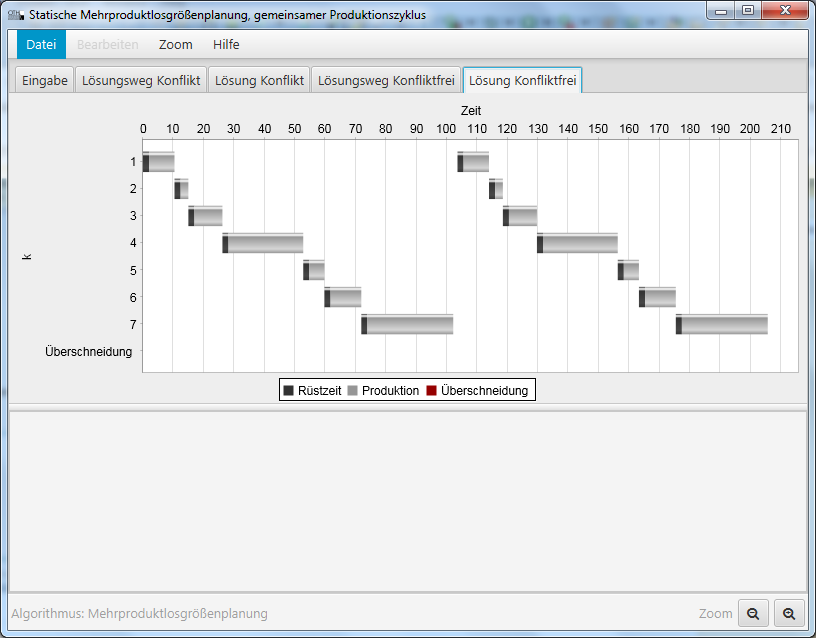
\includegraphics[width=0.8\linewidth]{Bilder/GanttMehrprodukt.png} 
	\captionof{figure}[Gantt Chart Mehrprodukt-Losgrößenplanung]{Gantt Chart- Graphische Darstellung der Lösungswerte der Mehrprodukt-Losgrößenplanung}
	\label{fig:mehrproduktgantt}
\end{figure}


\pagebreak

%-------------------------------------------------------------------------------------
% Verzeichnisse %-------------------------------------------------------------------------------------
	\rhead{Verzeichnisse} %Kopftextbeschriftung

	\stepcounter{section}
	\phantomsection \label{Verzeichnisse}
	\addcontentsline{toc}{section}{Verzeichnisse} %Ohne Nummer ins Inhaltsverzeichnis
	\renewcommand{\thesection}{\Roman{verzeichnis}}
	\section*{Verzeichnisse}
	% Literaturverzeichnis
	\rhead{Verzeichnisse}
	\renewcommand{\refname}{Literaturverzeichnis}
	\printbibliography
	\pagebreak
	
	% Abbildungsverzeichnis
	\stepcounter{verzeichnis}
	\listoffigures
	\pagebreak
	
	% Tabellenverzeichnis
	\stepcounter{verzeichnis}
	\listoftables
	\pagebreak
	
	% Abkürzungen
	\stepcounter{verzeichnis}
	\section{Abkürzungsverzeichnis}
	\vspace{-6em} % Abstand analog der anderen Verzeichnisse reduzieren
	\printnoidxglossary[type=\acronymtype,style=alttree,title=,toctitle=] %automatischen Titel und Gliederungsbeschriftung unterdrücken - sonst steht da Glossarie
	\newpage

% ---------------------------------------------------------------------------------
% Anhang
% ---------------------------------------------------------------------------------
\pagenumbering{Roman} %Seitennummerierung auf Romanisch stellen
\setcounter{page}{1}  %Seitenzähler initialisieren
\rhead{Anhang}        %Kopftextbeschriftung
\begin{appendix}
	\phantomsection \label{Anhang}
	\section*{Anhang}\addcontentsline{toc}{section}{Anhang} %Anhang ohne Nummer
	\renewcommand{\thesection}{\Roman{section}}
	
	\setcounter{section}{0} %Counter für Nummerirung der Anhänge initalisieren
	\section{Beispielimport}
	\label{app:beispielimport}
	Das hier aufgelistete Beispiel kann wie in Kapitel \ref{ch:programmeingaben} erklärt, über den Menüeintrag "'Datei"' importiert werden.

\subsection{Format}
Das Format der in den CSV-Dateien gespeicherten Produkte ist zweckmäßig gehalten. Die Werte aller Variablen eines Produkts befinden sich in derselben Zeile. Die Anzahl der Zeilen entspricht somit der Anzahl der zu importierenden Produkte. Die Reihenfolge der Variablenwerte pro Produkt ist folgende:
\begin{compactitem}
	\item Zeilenindex k
	\item Nachfragerate D
	\item Produktionsrate p
	\item Rüstzeit $\tau$
	\item Rüstkostensatz s
	\item Lagerkostensatz h
\end{compactitem}
Die einzelnen Werte werden dabei jeweils durch ein Semikolon voneinander getrennt.

\subsection{Beispiel: Fallstudie Tempelmeier}
Folgende Daten wurden aus \cite{Templ09} entnommen:
\begin{table}[H]
\begin{center}
\begin{tabular}{llllll}
\hline
\multicolumn{1}{|l|}{k} & \multicolumn{1}{l|}{$D_k$} & \multicolumn{1}{l|}{$p_k$} & \multicolumn{1}{l|}{${\tau}_k$} & \multicolumn{1}{l|}{$s_k$} & \multicolumn{1}{l|}{$h_k$} \\ \hline
1                       & 10.4                      & 128.5714                  & 2.0000                          & 190                       & 0.000689                  \\
2                       & 0.8                       & 32.43243                  & 2.0000                          & 210                       & 0.010280                  \\
3                       & 3.6                       & 40.44944                  & 2.0000                          & 140                       & 0.021853                  \\
4                       & 12.22222                  & 51.42857                  & 2.0000                          & 100                       & 0.005105                  \\
5                       & 2.666667                  & 55.38462                  & 2.0000                          & 150                       & 0.005920                  \\
6                       & 4                         & 40.90909                  & 2.0000                          & 110                       & 0.004753                  \\
7                       & 12.44444                  & 45.56962                  & 2.0000                          & 160                       & 0.003530                 
\end{tabular}
\caption[Daten aus \cite{Templ09}]{Daten aus \cite{Templ09}}
\end{center}
\end{table}
Der Inhalt der CSV-Datei hierzu sieht folgendermaßen aus:
\begin{figure}[H]
	\centering
	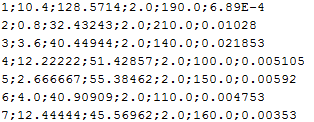
\includegraphics[width=0.5\linewidth]{Bilder/Export.png} 
	\captionof{figure}[Daten aus \cite{Templ09}]{Daten aus \cite{Templ09}}
	\label{fig:export}
\end{figure}

	
\end{appendix}
\end{document}
